

\section{Objetivo}
Que el alumno se familiarice con la abstracción del concepto de agente mediante la programación de un sistema de simulación biológico que muestra las bases de un autómata celular, programación dirigida a agentes, sistemas complejos y emergencia de propiedades como la auto-organización.\par


\begin{auxcode}
 \caption{Termitas}
 \centering
 \hurl{\auxprefix ia-termitas}
\end{auxcode}


\section{Introducci\'on}
\paragraph*{}
Un autómata celular es un modelo discreto que consiste en una cuadrícula de células, cada una con un número finito de estados. La cuadrícula puede estar en cualquier número finito de dimensiones pero lo más común es encontrar autómatas en una, dos y tres dimensiones para que tengan sentido geométrico. Cada célula tiene definido un conjunto de células llamado vecindad [\fref{fig:vecindadmoore} y ~\fref{fig:vecindadneumann}].


\begin{figure}
  \centering
  \begin{minipage}{.5\textwidth}
    \centering
    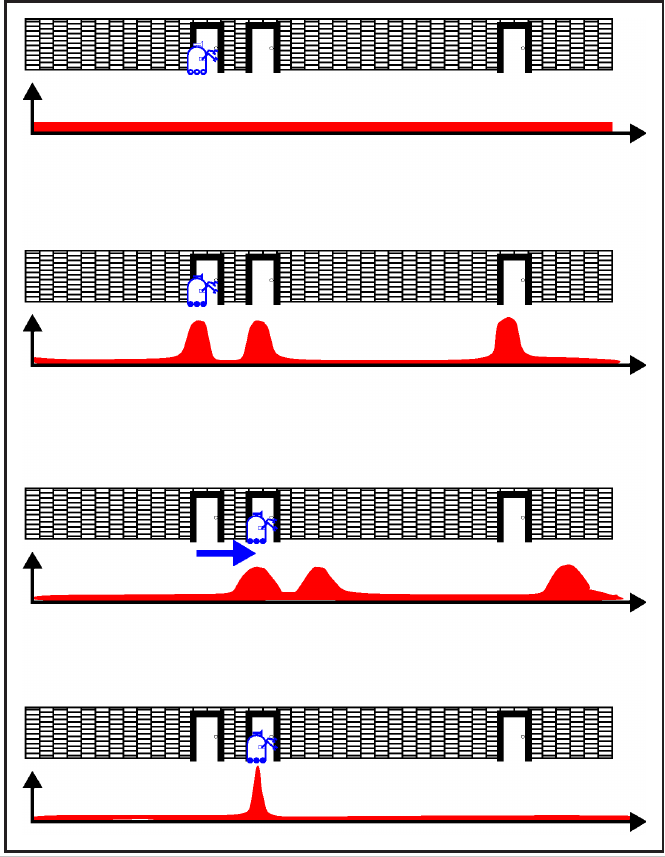
\includegraphics[width=.4\linewidth]{termitas/screen1.png}
    \captionof{figure}{Vecindad de Moore}
    \label{fig:vecindadmoore}
  \end{minipage}%
  \begin{minipage}{.5\textwidth}
    \centering
    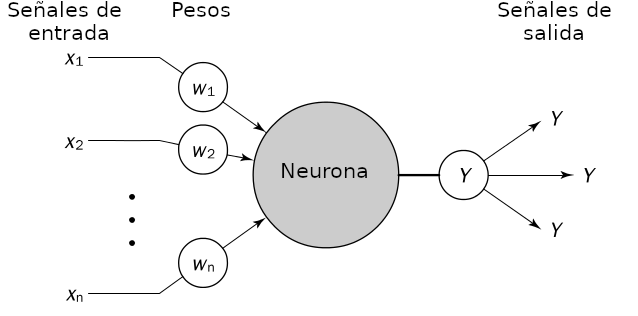
\includegraphics[width=.4\linewidth]{termitas/screen2.png}
    \captionof{figure}{Vecindad de Von Neumann de radio 1 (rojo) y radio 2 (rojo y rosa).}
    \label{fig:vecindadneumann}
  \end{minipage}
\end{figure}

Se tiene un estado inicial (al tiempo t=0) en el que se asigna un estado a cada célula. Una nueva generación es creada (avanzar t en 1) según alguna regla que determina el nuevo estado de cada célula en términos del estado actual de la célula y la de sus vecinos [\fref{fig:numtrans}].

\begin{figure}
  \centering
  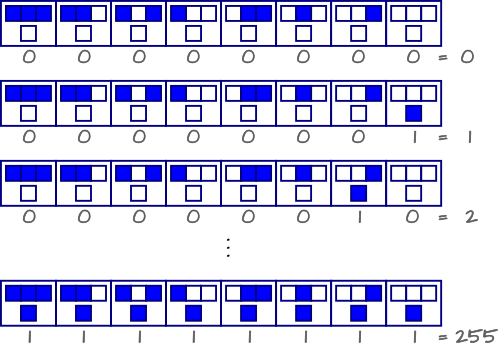
\includegraphics[width=0.6\textwidth]{termitas/Automata1D.png}
  \caption{Numeración de reglas de transición para autómatas celulares unidimensionales.}
  \label{fig:numtrans}
\end{figure}

\subsection{Modelo basado en agentes}
Un modelo basado en agentes es un tipo de modelo computacional que permite la simulación de acciones e interacciones entre individuos autónomos dentro de un entorno, y permite determinar qué efectos producen en el conjunto del sistema.\par

Combina elementos de teoría de juegos, sistemas complejos, emergencia, sociología computacional, sistemas multi-agente y programación evolutiva.
Los modelos simulan las operaciones simultáneas e interacciones de múltiples agentes, en un intento de recrear y predecir la apariencia de fenómenos complejos. El proceso de emergencia surge de un nivel bajo hacia niveles del sistema más altos. La clave es notar que reglas de comportamientos sencillos generan comportamientos complejos.\par


\subsection{Agentes aut\'onomos y auto-organizaci\'on}

Un agente autónomo es una unidad que interactúa con su entorno (el cual probablemente consta de otros agentes) pero actúa independientemente de todos los demás agentes porque no toma decisiones con respecto a algún líder o plan global a seguir. Es decir, cada agente actúa por sí mismo.\par

Así, veremos cómo múltiples agentes pueden desempeñar tareas que aparentan seguir un plan global. A este proceso en el que cada agente autónomo interactúa a su propia manera para crear un orden global se le conoce como auto-organización y se observa cómo modelos simples son capaces de generar comportamientos complejos.\par


\subsection{Modelo de termitas}

Mitchel \cite{Resnick1994} estudió varios sistemas de agentes primitivos, uno de ellos fueron las termitas teóricas dentro de un espacio con astillas esparcidas que seguían las siguientes reglas:

\begin{itemize}
  \item Caminar aleatoriamente hasta encontrar una astilla.
  \item Si la termita está cargando una astilla, la suelta y continua caminando aleatoriamente.
  \item Si la termina no está cargando una astilla, la toma y continua caminando aleatoriamente con la astilla.
\end{itemize}

Claramente, las reglas definidas por Resnick son tan simples como es posible. No parece haber lugar para un comportamiento inteligente en un modelo como éste, tampoco parece que las termitas puedan producir nada con algún sentido más allá de la aleatoriedad de las astillas distribuidas en el entorno.\par

La \fref{fig:termitasaleatorias} muestra seis escenarios de la simulación del conjunto de reglas simples con un conjunto pequeño de termitas. En la configuración inicial el universo de termitas consiste en una cuadrícula con astillas aleatoriamente distribuidas. La representación de la cuadrícula consta de una frontera periódica, es decir, un punto en una de las aristas de la cuadrícula tiene como vecinos a los puntos en la arista opuesta.
Al comenzar la simulación, las termitas mueven las astillas en pequeños grupos o clusters. Conforme pasa el tiempo, los clusters se vuelven más grandes y más definidos.\par

Tras cientos de miles de pasos en la ejecución de la simulación, como se muestra en la última imagen de la \fref{fig:termitasaleatorias}, las astillas están claramente bien definidas en una colección. Obviamente esto es un método poco óptimo para coleccionar astillas, sin mencionar lo frustrante que es observar el proceso. Sin embargo, con el paso del tiempo es un hecho que el orden del sistema es evidente como resultado.\par

\begin{figure}
  \centering
  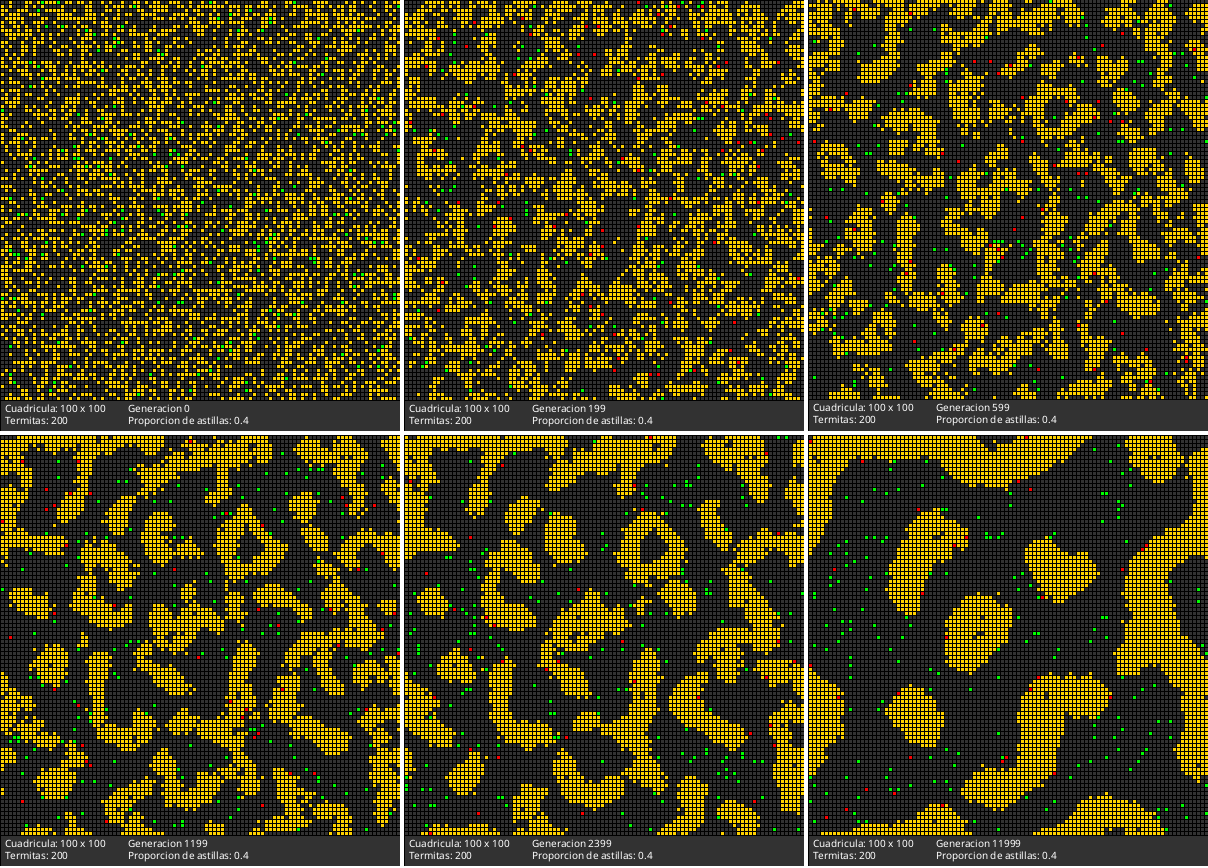
\includegraphics[width=0.9\textwidth]{termitas/Termitas.png}
  \caption{Termitas colocando aleatoriamente astillas con las reglas definidas anteriormente.  Reproducción del experimento en \cite{Resnick1994}.}
  \label{fig:termitasaleatorias}
\end{figure}



\section{Desarrollo e implementaci\'on}


Los resultados anteriores son reportados por el propio Resnick, sin embargo, para mostrar que es posible llegar al mismo resultado, se lleva a cabo una implementación con el lenguaje de programación \classname{Processing}.
Al alumno se le proporciona parte de la implementación, de manera que se enfoque únicamente en programar el comportamiento descrito y evitando perder tiempo en la interfaz gráfica.

Las clases, métodos y variables más relevantes son las siguientes:

\begin{description}%[leftmargin=40pt, labelindent=20pt]
  \item[Clase Celda] \hfill \\
    Representación de cada espacio dentro de la cuadrícula donde estarán las termitas y astillas.
    Cada celda tiene coordenadas (x,y) y un valor booleano para indicar si hay una astilla.

  \item[Clase Termita] \hfill \\
    Representación de una termita. Se representan las coordenadas (x,y) de su posición, la dirección en la que está observando (auxiliar que más adelante será mencionado a detalle) y un valor booleano para indicar si está cargando una astilla.

  \item[Clase ModeloTermitas] \hfill \\
    Representación de una colonia de termitas. Principalmente contiene una matriz de celdas (la representación del mundo) y una lista de termitas (nuestros agentes). Adicionalmente se define la cantidad de celdas a lo ancho y alto, un valor auxiliar para conocer la cantidad de iteraciones, un objeto de la clase Random (para hacer decisiones aleatorias) y el tamaño en pixeles de cada celda (para la visualización con Processing).
\end{description}

\subsection{Implementaci\'on}

Para reproducir el experimento de \cite{Resnick1994} haremos uso del lenguaje de programación \Java, pero nos auxiliaremos de la biblioteca \code{core.jar} del lenguaje \code{Processing}\footnote{\hurl{https://processing.org/}}.  Esto nos permitirá crear el ambiente gráfico al heredar de la clase
\begin{center}
 \code{processing.core.PApplet}.
\end{center}
De esta clase sobreescribimos tres métodos:
\begin{itemize}
 \item \code{setup} Permite configurar el fondo de la ventana y crear los objetos que se utilizarán durante la ejecución de la animación.

 \item \code{settings} Aquí se hacen configuraciones iniciales como el tamaño de la ventana a mostrar.

 \item \code{draw} Método que es llamado periódicamente en el hilo de procesamiento y desde el cual se actualiza el contenido a mostrar.
\end{itemize}

El código auxiliar para esta práctica ya muestra cómo generar una animación inicial.  El constructor de la clase \classname{ModeloTermitas} ya está implementado (principalmente para inicializar el espacio y termitas). También se encuentra implementado el método \classname{moverTermita}, que mueve la termita dada como parámetro en la dirección indicada. Cada termita tiene una vecindad de Moore, es decir, tienen 8 celdas adyacentes (considerando un espacio periódico) que se enumeran según la \fref{fig:dirsposibles1}.

\begin{figure}
  \begin{center}
    \begin{tabular}{| l | c | r |}
      \hline
      0 & 1 & 2 \\ \hline
      7 &   & 3 \\ \hline
      6 & 5 & 4 \\
      \hline
    \end{tabular}
  \end{center}
  \caption{Las 8 posibles direcciones y vecindades de cada termita o celda.}
  \label{fig:dirsposibles1}
\end{figure}

De la misma manera se indica la dirección en la que puede mirar una termita. Por ejemplo, si la termita está mirando en dirección con valor 1 significa que está observando hacia arriba. Si tuviera el valor 4 significa que está observando en diagonal inferior derecha.

Existen 3 maneras diferentes de simular e implementar el modelo de termitas:

\begin{enumerate}
  \item \textbf{Usando las 8 posibles direcciones} \\
    Siguiendo la idea original con caminatas aleatorias en las 8 posibles direcciones para las termitas.


  \item \textbf{Modificar la caminata para que sea aleatoria y restringida} \\
    Una manera de avanzar totalmente aleatoria como en el primer caso implica que pueden existir muchos movimientos innecesarios (considerese la situación en la que una termita se cicla moviéndose en la casilla delante de ella y detrás de ella).
    Empleando la dirección en la que está observando la termita se puede restringir su movimiento a solo 3 opciones: a la izquierda, al frente o a la derecha.
    Adicionalmente al soltar una astilla, la termita da media vuelta y se coloca en la dirección opuesta de donde soltó la astilla (esto evita una situación similar en la que se cicle una termita moviendo la misma astilla al mismo lugar).

  \item \textbf{Brindar un salto a las termitas} \\
    Esto significa que en el momento en que una termita suelta una astilla, en lugar de moverse en la dirección opuesta, las termitas “brincan” o se mueven a una celda sin astilla y continúan caminando de manera aleatoria y restringida.
\end{enumerate}

Cada una de las diferentes maneras de implementación se encuentran asignadas a los métodos \classname{evolucion1}, \classname{evolucion2} y \classname{evolucion3}, respectivamente.

El archivo \classname{termitas/Termitas.java} contiene parte del código de la simulación y solamente tiene implementada la visualización de las termitas como cuadrados verdes moviéndose aleatoriamente [\fref{fig:sinastillas}]. Al implementar todos los métodos faltantes se darán cuenta de que cuando una termita está cargando una astilla (cuadros amarillos) cambia de color a rojo.


% Fig. 6. Captura de pantalla del código Termitas.pde de Processing
\begin{figure}
  \centering
  \includegraphics[width=0.7\textwidth]{termitas/sinastillas.png}
  \caption{Captura de pantalla de \classname{Termitas.java}, que hace uso de Processing.}
  \label{fig:sinastillas}
\end{figure}

Se debe implementar el comportamiento de las termitas para simular todo el sistema de la mejor manera. Dado que la interfaz gráfica está dada, solamente es necesario implementar los siguientes métodos:

\begin{itemize}
  \item \classname{int direccionAleatoriaFrente(int direccion)}
  \item \classname{boolean hayAstilla(Termita t, int direccion)}
  \item \classname{void dejarAstilla(Termita t, int direccion)}
  \item \classname{void dejarAstilla(Termita t)}
  \item \classname{void dejarAstillaConSalto(Termita t)}
  \item \classname{void tomarAstilla(Termita t, int direccion)}
\end{itemize}

Cada método se encuentra especificado dentro del archivo \classname{Termitas.java}.


\section{Requisitos y resultados}

Para evaluar y calificar la práctica es necesario que se implementen todos los métodos mencionados e indicados en el código, respetando implementar sólo lo que se pide (para evitar comportamientos extraños de la simulación).
Es completamente válido utilizar bibliotecas adicionales si lo consideran necesario, así como la creación y uso de sus propios métodos auxiliares si lo desean.

Debe notarse una mejora significativa mediante la implementación de la caminata restringida o el uso del salto. Es decir, verifiquen que tras varias iteraciones su implementación del modelo actúe como se espera. Las siguientes imágenes ilustran parte de los resultados esperados [Figuras ~\ref{fig:evo1}, ~\ref{fig:evo2} y ~\ref{fig:evo3}].

\begin{figure}
  \centering
  \includegraphics[width=0.65\textwidth]{termitas/evo1.png}
  \caption{Simulación con idea original después de 10000 iteraciones (evolucion1).}
  \label{fig:evo1}
\end{figure}

\begin{figure}
  \centering
  \includegraphics[width=0.65\textwidth]{termitas/evo2.png}
  \caption{Empleando caminata aleatoria restringida tras 5000 iteraciones. La cantidad de astillas es la misma pero se observa un mejor ordenamiento y en menor tiempo.}
  \label{fig:evo2}
\end{figure}

\begin{figure}
  \centering
  \includegraphics[width=0.65\textwidth]{termitas/evo3.png}
  \caption{El uso de termitas con salto brinda una aproximación similar a la anterior. Cambiando algunos parámetros se pueden obtener resultados similares a colonias de termitas de la naturaleza.}
  \label{fig:evo3}
\end{figure}

% \subsection{Agradecimientos}
% \noindent Esta práctica fué realizada originalmente por Rodrigo Eduardo Colín Rivera (animeroy@gmail.com), las modificaciones hechas fueron mínimas, por lo que todo el crédito va para el. \\\\


% \begin{figure}[h]
%   \centering
%   \includegraphics[width=0.65\textwidth]{evo1.png}
%   \caption{Simulación con idea original después de 10000 iteraciones (evolucion1).}
%   \label{fig:evo1}
% \end{figure}

% \begin{figure}[h]
%   \centering
%   \includegraphics[width=0.65\textwidth]{evo2.png}
%   \caption{Empleando caminata aleatoria restringida tras 5000 iteraciones. La cantidad de astillas es la misma pero se observa un mejor ordenamiento y en menor tiempo.}
%   \label{fig:evo2}
% \end{figure}

% \begin{figure}[h]
%   \centering
%   \includegraphics[width=0.65\textwidth]{evo3.png}
%   \caption{El uso de termitas con salto brinda una aproximación similar a la anterior. Cambiando algunos parámetros se pueden obtener resultados similares a colonias de termitas de la naturaleza.}
%   \label{fig:evo3}
% \end{figure}

